\section{Background}\label{sec:background}
The influence of hardware faults on DNN acceleration system is closely related with 
the micro architecture of DNN accelerators. To investigate the fault tolerance 
of a DNN acceleration system, we take a typical DNN accelerator with a regular 
2D processing element (PE) array as an example and elaborate its architecture 
in this section.

The representative DNN accelerator is illustrated in 
Figure ~\ref{fig:npu-arch}. It adopts output stationary data flow 
to map computing such as convolution to the 2D processing element (PE) array. 
Each PE in the array performs all the operations required to yield 
an output activation. It has a single multiplier and accumulator 
to convolve the input activations from all the different channels 
for an output sequentially. To that end, weights 
are fed to the first column of the PE array in parallel and flow 
through PEs from left to right to ensure that all PEs operate in full 
scale. While input activations are organized in a batch and broadcast 
to one column of PE every cycle, each PE in the column shares the 
same input data and it takes each PE multiple cycles to consume the 
the batched data. During this period, more batched input activations 
can be read and sent to the next column of PEs along with 
the movement of the weights. Output activations flow 
from right to left in column-wise. Eventually, each row of the PEs
array produces a set of sequential output activations in 
the same row of one output feature map on y-axis. 
Each column of the PEs produces the output activations 
belonging to different output feature maps. 
The architecture along with the compact data flow achieves 
high data reuse under limited on-chip buffer bandwidth provision. 

\begin{figure}
    \center{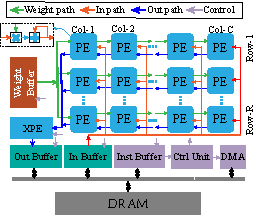
\includegraphics[width=0.7\linewidth]{npu-arch}}
    \caption{Typical DNN accelerator architecture with regular 2D PE array}
\vspace{-0.5em}
\label{fig:npu-arch}
\end{figure}

Both convolution layer and full connection layer can be mapped to the 
array efficiently. While pooling and other non-linear activation functions 
such as sigmoid will be performed right after the computing-intensive 
layers like convolution layer in a module named XPE such that 
the data movement between the two layers can be reduced. 
All the neural network operations can be mapped to the 
accelerator. To map diverse neural network models with different 
combination of layers and parameters such as 
stride size, kernel size, and input/output feature map size, we define 
a set of instructions to generate appropriate control signals 
for different neural network operations. Each neural network 
will be compiled to a series of instructions and executed sequentially. 
In addition, neural network input features and weights 
are usually larger than the on-chip buffers and PE array size, 
so they must be tiled and the tiles need to be scheduled to 
obtain efficient execution on the accelerator. To enable fine-grained 
optimizations, each instruction only handles operations of 
a single tile. Thus, tiling is performed during model
compilation and it is transparent to the instructions.

Table \ref{tab:instrction-set} shows the instruction set of the neural 
network accelerator. It adopts 64-bit fixed length encoding 
and consists of three types of instructions including calculation, 
data movement and control. The calculation instruction  
category defines the input/output feature size, kernel size, 
Q-code, and DMA parameter and it includes different operations 
used in neural networks such as convolution, full connection, 
pooling, addition, softmax, dot-accumulation and activation 
function etc. Since some of the calculation instructions have too 
many parameters to fit to the 64bit instruction, they are split 
into two consecutive ones and executed as a single one. 
Data movement category includes three instructions which move a block of data 
from DRAM to buffer, buffer to DRAM and buffer to buffer 
respectively. Finally, control category includes three instructions which are 
Jump, Stop and Nop. Jump instruction is mainly used for repeated 
execution. Stop is used to terminate the execution of the accelerator.
Nop is used to resolve the data dependency between sequential 
instructions.

\begin{table}
    \centering
    \caption{Instruction Set of the DNN Accelerator}
    \label{tab:instrction-set}
    \begin{tabular}{cp{0.6\columnwidth}}
        \toprule
        Instruction Type & Description \\
        \midrule
        Calculation & Setup parameters for the computing operations such as 
        the input/output feature size, kernel size, Q-code, and
        performs various neural network operations such as convolution, full 
        connection, pooling, addition, softmax, dot-accumulation and activation 
        function \\
        \midrule
        Data movement & Move a block of data from buffer to buffer, buffer to DRAM and DRAM to buffer.\\
        \midrule
        Control & Control the execution of the accelerator such as Jump, Nop and Stop\\
    \bottomrule
    \end{tabular}
    \vspace{-1em}
\end{table}

The neural network accelerator architecture is designed to be general to support 
various neural network models. In addition, it typically works along 
with a general purposed processor and allows configuration as well as 
controlling from the attached processor. It assumes that
the input data, weight and output data are stored in DRAM which can be 
accessed directly.
